\documentclass[MIOP.tex]{subfiles}
\usepackage{mathtools}
\begin{document}

\chapter{Introducción a la Programación\\ Dinámica.}
\section{Introducción.}
La Programación Dinámica (P.D.) es un conjunto de técnicas que permiten resolver procesos de división secuencial.
\begin{ej}
Probabilidad de que al lanzar dos dados sucesivamente tengan antes un suceso que sume 3 a uno que sume 7. Llamemos $A=$``obtener un suceso que sume 3 antes que uno que suma 7''. Tratamos de expresar la probabilidad recursivamente. 

$P(A)=P(A/1er$ lanzamiento suma $3)P(1er$ lanzamiento suma 3$)+P(A/1er$ lanzamiento suma $7)P(1er$ lanzamiento suma $7)+P(A/1er$ lanzamiento no suma ninguno$)P(1er$ lanzamiento no suma ninguno$)$. Sustituyendo por su valor:
$$P(A)=1\cdot\frac{2}{36}+0\cdot\frac{6}{36}+P(A)\frac{28}{36}=\frac{2}{36}+P(A)\frac{28}{36}.$$
Podemos despejar y obtenemos $P(A)=\dfrac{1}{4}$. 
\end{ej}

\begin{ej}
Calcular el factorial de un número recursivamente. Entonces $f(n)=n!=nf(n-1)$. Si sabemos que $f(0)=1$ podemos calcularla para cualquier $n\in\N$.
\end{ej}

\begin{ej} Calcular el camino más corto para ir de $1$ hasta $7$. Para llegar al nodo $7$, necesariamente hay que pasar por uno de los $3$ a los que está conectado. Llamamos $l_{ij}$ a la longitud del arco $(i,j)$. Si definimos $f(i)=$``longitud del camino más corto desde $i$ hasta $7$''. Sabemos que $f(7)=0$. 
\[
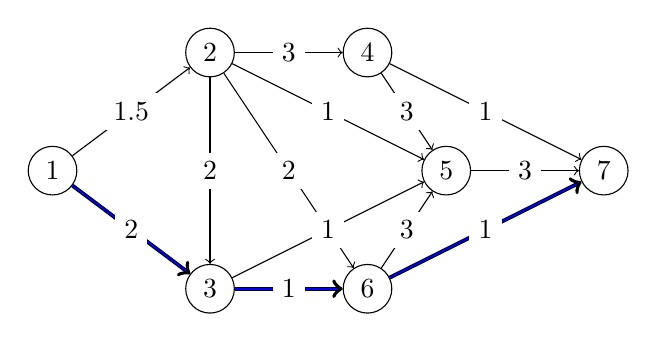
\begin{tikzpicture}
    \node[shape=circle,draw=black] (A) at (0,1.5) {$1$};
    \node[shape=circle,draw=black] (C) at (2,0) {$3$};    
    \node[shape=circle,draw=black] (B) at (2,3) {$2$};
    \node[shape=circle,draw=black] (D) at (4,3) {$4$};
    \node[shape=circle,draw=black] (E) at (4,0) {$6$};
    \node[shape=circle,draw=black] (F) at (5,1.5) {$5$};
    \node[shape=circle,draw=black] (G) at (7,1.5) {$7$};
\tikzset{mystyle/.style={->,double=blue}} 
\tikzset{every node/.style={fill=white}} 
     \path [->] (A) edge node {$1.5$} (B);
     \path [->] (A) edge [mystyle]  node {$2$} (C);
     \path [->] (B) edge node {$2$} (C);
     \path [->] (B) edge node {$1$} (F);
     \path [->] (B) edge node {$2$} (E);
     \path [->] (B) edge node {$3$} (D);
     \path [->] (C) edge [mystyle]  node {$1$} (E);
     \path [->] (C) edge node {$1$} (F);
     \path [->] (D) edge node {$3$} (F);
     \path [->] (D) edge node {$1$} (G);
     \path [->] (E) edge [mystyle] node {$1$} (G);
     \path [->] (F) edge node {$3$} (G);
	 \path [->] (E) edge node {$3$} (F);
\end{tikzpicture}
\]
\begin{align*}
f(4)=&\min\{l_{47},l_{45}+f(5)\}=\min\{1,6\}=1\\
f(5)=&\min\{l_{57}\}=3\\
f(6)=&\min\{l_{67},f(5)+l_{65}\}=\min\{1,3+3\}=1\\
f(3)=&\min\{l_{35}+f(5),l_{36}+f(6)\}=\min\{1+3,1+2\}=3\\
f(2)=&\min\{l_{24}+f(4),l_{25}+f(5),l_{26}+f(6),l_{23}+f(3)\}=\min\{3+1,1+3,2+1,2+2\}=3\\
f(1)=&\min\{l_{12}+f(2),l_{13}+f(3)\}=\min\{1.5+3,2+2\}=4
\end{align*}

Tenemos que el camino más corto tiene longitud $4$ y se corresponde con el camino $1->3->6->7$. Sea $\Gamma(i)=\{j:\exists (i,j)$ en el grafo$\}$. Entonces $f(7)=0$ y $f(i)=\min_{j\in\Gamma(i)}\{l_{ij}+f(j)\}\forall j\neq 7$.

\end{ej}

\subsection{Elementos de P.D.}
\begin{enumerate}
\item El problema se puede descomponer en subproblemas (etapas) y debemos tomar una decisión en cada uno de ellos.
\item En cada etapa hay un número finito de estados.
\item La decisión que se realiza en un estado determina la transición al estado en la etapa siguiente.
\item En un estado, la decisión óptima de los problemas en etapas futuras no depende de las decisiones anteriores. 
\item Debe existir un funcional $f$ que relacióna el valor de un subproblema en la etapa $k$ con el de la etapa $k+1$ (o $k-1$). 
\end{enumerate}

Denotemos por $s_k$ la variable que denota el estado en la etapa $k$. Sea $d_k$ una decisión factible en el estado $s_k$ y $c_k(s_k,d_k)$ el coste incurrido en el estado $k$ si se decide $d_k$. Asimismo, sea $t_k(s_k,d_k)$ el estado al que evoluciona el sistema en la etapa $k+1$ si en $s_k$ se decide $d_k$.

Usando el ejemplo anterior:
\begin{itemize}
\item $s=$nodo.
\item decisiones: $d\in\Gamma(i)$.
\item $c(i,d)=l_{id}$.
\item $t(i,d)=d$.
\end{itemize}

\textbf{Diagrama de cajas}
Etapa $k$:
$\overset{d_k}{\longrightarrow}\boxed{s_k}\rightarrow c_k(s_k,d_k)$\\
Etapa $k+1$:
$\overset{d_k}{\longrightarrow}\boxed{t_k(s_k,d_k)}\rightarrow c_k(s_{k+1},d_{k+1})$

\begin{defi}
Sea $g:\R^n\to\R$. Decimos que $g$ es \textbf{separable} si $\exists g_1:\R^2\to\R,g_2:\R^{n-1}\to\R$ tales que $g(u_1,u_2,\dots,u_n)=g_1(u_1,g_2(u_2,\dots,u_n))$. 
\end{defi}

\begin{defi}
$g:\R^n\to\R$ es \textbf{descomponible} si
\begin{enumerate}
\item Es separable con $g_1,g_2$ y
\item $g_1$ es monótona no creciente como función de $g_2$ (en proceso de minimización, no decreciente si es maximización). 
\end{enumerate}
\end{defi}

\begin{ej}
Suma, producto de números positivos, máximo... 
\end{ej}

\begin{teorema}[Mitten] 
Sea $g:\R^n\to\R$ una función descomponible en $g_1,g_2$. Asumimos que nos movemos en dominios compactos y las funciones son continuas, de modo que se alcanzan los mínimos. Entonces se verifica:
$$\min_{r_1,r_2,\dots,r_n} g(r_1,r_2,\dots,r_n)=\min_{r_1} g_1(r_1,\min_{r_2,\dots,r_n}g_2(r_2,\dots,r_n))$$

\end{teorema}
\begin{dem}
Dado que $\forall u_1,\dots, u_n$ $g(u_1,\dots, u_n)=g_1(u_1,g_2(u_2,\dots, u_n))$. Entonces 
$$\min_{r_1,\dots,r_n}g(r_1,\dots,r_n)\leq g_1(u_1,g_2(u_2,\dots, u_n))\;\forall u_1,u_2,\dots,u_n.
$$ 
Por tanto, 
$$\min_{r_1,\dots,r_n}g(r_1,\dots,r_n)\leq g_1(u_1,\min_{u_2,\dots,u_n}g_2(u_2,\dots, u_n))\forall u_1.$$ 
Luego 
$$\min_{r_1,\dots,r_n}g(r_1,\dots,r_n)\leq \min_{u_1}g_1(u_1,\min_{u_2,\dots,u_n}g_2(u_2,\dots, u_n))$$
Análogamente, usando que $g_1$ es no creciente en $g_2$, $$g(u_1,\dots, u_n)\geq g_1(u_1,\min_{r_2,\dots,r_n}g_2(r_2,\dots,r_n))\forall u_1.$$ Por consiguiente, 
$$g(u_1,\dots, u_n)\geq \min_{r_1}g_1(r_1,\min_{r_2,\dots,r_n}g_2(r_2,\dots,r_n)).$$ Finalmente,
$$\min_{u_1,\dots,u_n}g(u_1,\dots, u_n)\geq \min_{r_1}g_1(r_1,\min_{r_2,\dots,r_n}g_2(r_2,\dots,r_n)).$$\QED
\end{dem}

\section{Ecuaciones de un proceso de decisión.}
Consideremos un proceso de decisión secuencial en $N$ etapas y denotemos por $s_n$ el estado en la etapa $n$. Supongamos que conocemos el estado final del proceso $s_N^*$. Sean $c_n(s_n,d_n)$ y $t_n(s_n,d_n)$, respectivamente, las funciones de coste y transición entre etapas. Finalmente, supongamos que $f_n(s_n)$ representa el menor coste para ``conducir'' al sistema desde la etapa $n$ en estado $s_n$ hasta $s_N^*$. Entonces, podemos escribir $f_n(s_n)=\min_{d_n}\{c_n(s_n,d_n)+f_{n+1}(t_n(s_n,d_n))\}$ para $n<N$. Y para $n=N$, $f_N(s_N)=\begin{cases}
+\infty & s_N\neq s_N^*\\
\min_{d_N}c_N(s_N^*, d_N) & s_N=s_N^*
\end{cases}$

Estas ecuaciones se pueden extender a otras funciones $g$ siempre que sean descomponibles.
$f_n(s_n)=\min_{d_n}\{g_1(c_n(s_n,d_n)),f_{n+1}(t_n(s_n,d_n))\}$.
\begin{ejer}[Problema de producción e inventario]
Consideremos un proceso de producción en $T$ etapas, $t=1,2\dots,T$. En la etapa $t$ existe una demanda $d_t$ que hay que satisfacer. En cada etapa se puede decidir producir $x$ unidades  con un coste $c_t(x)$. Además existe un coste de almacén $h_t(I_t)$, que representa el coste en el periodo $t$ por tener $I_t$ unidades al comienzo de este periodo. Suponemos que $I_1=0=I_{T+1}$.  En estado $I_t$, $f_t(I_t)$ es el mínimo coste para atender la demanda desde $t$ a $T$ si en $t$ tengo $I_t$ en inventario. Entonces $f_t(I_t)=\min_{x_t}\{c_t(I_t,x_t)+f_{t+1}(I_t+x-d_t)+h_t(I_t)\}$ si $t<T+1$ y $f_{T+1}=\begin{cases}
+\infty & I_{T+1}>0\\
0 & I_{T+1}=0
\end{cases}$

Donde $x_t$ son las unidades producidas en la etapa $t$ y $d_t$ la demanda en la etapa $t$. La solución del problema es $f_1(0)$. Resolver el problema con los siguientes datos.

\begin{tabular}{|c| c c c c|}
\hline
$t$ & $1$ & $2$ & $3$ & $4$\\
\hline
$d_t$ & $1$ & $3$ & $2$ & $4$\\
\hline

\end{tabular}

$I_1=I_5=0$, $h_t(I)=\frac{1}{2}I$ ($I\leq 4$), $c_t(x)=\begin{cases}
3+x & 5\geq x>0\\
0 & x=0
\end{cases}$
\end{ejer}
\begin{solucion}
\underline{Etapa 4:}\

\begin{tabular}{|c| c| c| c |}
\hline
$I$ & $x$ & $f_4(I)$ \\
\hline
$0$ & $4$ & $7$   \\
\hline
$1$ & $3$ & $\frac{1}{2}1+6$  \\
\hline
$2$ & $2$ & $\frac{1}{2}2+5$  \\
\hline
$3$ & $1$ & $\frac{1}{2}3+4$   \\
\hline
$4$ & $0$ & $\frac{1}{2}4+0$ \\
\hline
\end{tabular}\
\\

\underline{Etapa 3:}\kern 18.85em \underline{Etapa 2:}

\begin{tabular}{|c| c| c| c | c| c|}
\hline
$I$ & $x$ & $\frac{1}{2}I+c(x)$ & $f_4(I-2+x)$ &  $f_3(I)$ & $x^* $ \\
\hline
$0$ & $2$ & $5$ & $7$  & $12$& $\boxed{2}$\\
\hline
 & $3$ & $0+6$ &$6,5$ & $12,5$ &\\
\hline
 & $4$ & $0+7$ & $6$ & $13$&\\
\hline
 & $5$ & $0+8$ & $5,5$ & $13,5$ & \\
\hline
\hline
$1$ & $1$ & $\frac{1}{2}+4$ & $7$  & $11,5$& $\boxed{1}$\\
\hline
 & $2$ & $\frac{1}{2}+5$ &$6,5$ & $12$ &\\
\hline
 & $3$ & $\frac{1}{2}+6$ & $6$ & $12,5$&\\
\hline
 & $4$ & $\frac{1}{2}+7$ & $5,5$ & $13$ & \\
\hline
 & $5$ & $\frac{1}{2}+8$ & $2$ & $13,5$ & \\
\hline
\hline
$2$ & $0$ & $\frac{1}{2}2+0$ & $7$  & $8$& $\boxed{0}$\\
\hline
 & $1$ & $\frac{1}{2}2+4$ &$6,5$ & $11,5$ &\\
\hline
 & $2$ & $\frac{1}{2}2+5$ &$6$ & $12$ &\\
\hline
 & $3$ & $\frac{1}{2}2+6$ & $5,5$ & $12,5$&\\
\hline
 & $4$ & $\frac{1}{2}2+7$ & $2$ & $10$ & \\
\hline
\hline
$3$ & $0$ & $\frac{1}{2}3+0$ & $6,5$  & $8$ & $\boxed{0}$\\
\hline
 & $1$ & $\frac{1}{2}3+4$ &$6$ & $11,5$ &\\
\hline
 & $2$ & $\frac{1}{2}3+5$ &$5,5$ & $12$ &\\
\hline
 & $3$ & $\frac{1}{2}3+6$ & $2$ & $9,5$&\\
 \hline
 \hline
 $4$ & $0$ & $\frac{1}{2}4+0$ & $6$  & $8$& $\boxed{0}$\\
\hline
 & $1$ & $\frac{1}{2}4+4$ &$5,5$ & $11,5$ &\\
\hline
 & $2$ & $\frac{1}{2}4+5$ &$2$ & $9$ &\\
 \hline
\end{tabular}\quad 
\begin{tabular}{|c| c| c| c | c| c|}
\hline
$I$ & $x$ & $\frac{1}{2}I+c(x)$ & $f_3(I-3+x)$ &  $f_2(I)$ & $x^* $ \\
\hline
$0$ & $3$ & $0+6$ &  $12$  & $18$& \\
\hline
 & $4$ & $0+7$ &$11,5$ & $18,5$ &\\
\hline
 & $5$ & $0+8$ & $8$ & $16$& $\boxed{5}$\\
\hline
\hline
$1$ & $2$ & $\frac{1}{2}+5$ & $12$  & $17,5$& \\
\hline
 & $3$ & $\frac{1}{2}+6$ &$11,5$ & $18$ &\\
\hline
 & $4$ & $\frac{1}{2}+7$ & $8$ & $15,5$& $\boxed{4}$\\
\hline
 & $5$ & $\frac{1}{2}+8$ & $8$ & $16,5$ & \\
\hline
\hline
$2$ & $1$ & $\frac{1}{2}2+4$ & $12$  & $17$& \\
\hline
 & $2$ & $\frac{1}{2}2+5$ &$11,5$ & $17,5$ &\\
\hline
 & $3$ & $\frac{1}{2}2+6$ &$8$ & $15$ &$\boxed{3}$\\
\hline
 & $4$ & $\frac{1}{2}2+7$ & $8$ & $16$&\\
\hline
 & $5$ & $\frac{1}{2}2+8$ & $8$ & $17$ & \\
\hline
\hline
$3$ & $0$ & $\frac{1}{2}3+0$ & $12$  & $13,5$ & $\boxed{0}$\\
\hline
 & $1$ & $\frac{1}{2}3+4$ &$11,5$ & $17$ &\\
\hline
 & $2$ & $\frac{1}{2}3+5$ &$8$ & $14,5$ &\\
\hline
 & $3$ & $\frac{1}{2}3+6$ & $8$ & $15,5$&\\
 \hline
 & $4$ & $\frac{1}{2}3+7$ & $8$ & $16,5$&\\
 \hline
 \hline
 $4$ & $0$ & $\frac{1}{2}4+0$ & $13,5$  & $8$& $\boxed{0}$\\
\hline
 & $1$ & $\frac{1}{2}4+4$ &$8$ & $14$ &\\
\hline
 & $2$ & $\frac{1}{2}4+5$ &$8$ & $15$ &\\
 \hline
  & $3$ & $\frac{1}{2}4+6$ &$8$ & $16$ &\\
 \hline
\end{tabular}\
\\

\underline{Etapa 1:}\

\begin{tabular}{|c| c| c| c | c| c|}
\hline
$I$ & $x$ & $\frac{1}{2}I+c(x)$ & $f_2(I-1+x)$ &  $f_1(I)$ & $x^* $ \\
\hline
$0$ & $1$ & $0+4$ &  $16$  & $20$& $\boxed{1}$ \\
\hline
 & $2$ & $0+5$ &$15,5$ & $20,5$ &\\
\hline
 & $3$ & $0+6$ & $15$ & $21$& \\
 \hline
 & $4$ & $0+7$ & $13,5$ & $20,5$& \\
 \hline
 & $5$ & $0+8$ & $13,5$ & $21,5$& \\
\hline
\end{tabular}\

Partiendo del óptimo en la etapa $1$, construimos la solución general que es
$$x_1=1,x_2=5,x_3=0,x_4=4.$$
\end{solucion}
\subsection{Una reformulación alternativa}
Consideremos un grafo $(V,E)$ donde los nodos de $V$ son de la forma $(n,i)$, siendo $n$ la etapa del proceso, e $i$ el nivel inicial de inventario en esa etapa. Los arcos del grafo existen entre $(n,i)$ y $(n+1,i-d_n+x)$ $\forall x$ factible, y su coste cendrá dado por $h_n(i)+c_n(x)$. 

\[
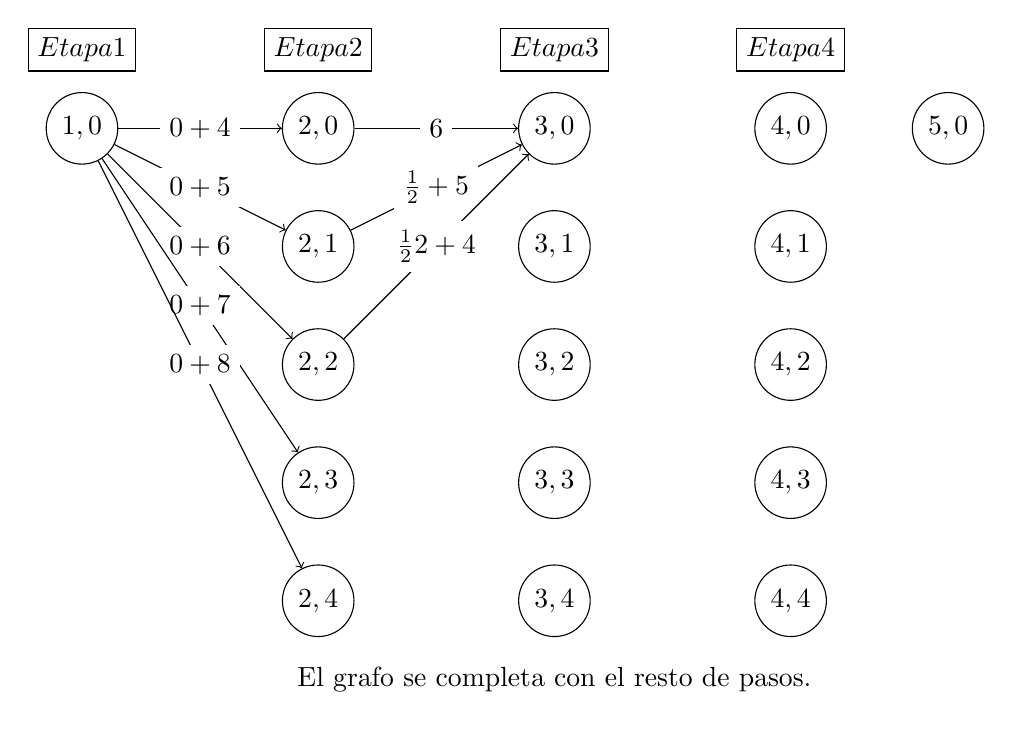
\begin{tikzpicture}
 	\node[shape=rectangle,draw=black] (Z) at (-4,4) {$Etapa 1$};
 	\node[shape=rectangle,draw=black] (Y) at (-1,4) {$Etapa 2$};
 	\node[shape=rectangle,draw=black] (X) at (2,4) {$Etapa 3$};
 	\node[shape=rectangle,draw=black] (W) at (5,4) {$Etapa 4$};
 	
    \node[shape=circle,draw=black] (A) at (-4,3) {$1,0$};
    \node[shape=circle,draw=black] (B) at (-1,3) {$2,0$};
    \node[shape=circle,draw=black] (C) at (2,3) {$3,0$};
    \node[shape=circle,draw=black] (D) at (5,3) {$4,0$};  
      
    \node[shape=circle,draw=black] (E) at (7,3) {$5,0$}; 
    
    \node[shape=circle,draw=black] (B1) at (-1,1.5) {$2,1$};
    \node[shape=circle,draw=black] (C1) at (2,1.5) {$3,1$};
    \node[shape=circle,draw=black] (D1) at (5,1.5) {$4,1$};
    
    \node[shape=circle,draw=black] (B2) at (-1,0) {$2,2$};
    \node[shape=circle,draw=black] (C2) at (2,0) {$3,2$};
    \node[shape=circle,draw=black] (D2) at (5,0) {$4,2$};
    
    \node[shape=circle,draw=black] (B3) at (-1,-1.5) {$2,3$};
    \node[shape=circle,draw=black] (C3) at (2,-1.5) {$3,3$};
    \node[shape=circle,draw=black] (D3) at (5,-1.5) {$4,3$};
    
    \node[shape=circle,draw=black] (B4) at (-1,-3) {$2,4$};
    \node[shape=circle,draw=black] (C4) at (2,-3) {$3,4$};
    \node[shape=circle,draw=black] (D4) at (5,-3) {$4,4$};
    
    \node[draw=none, fill=none] (NOTA) at (2,-4) {$\text{El grafo se completa con el resto de pasos.}$};

\tikzset{every node/.style={fill=white}} 
     \path [->] (A) edge node {$0+4$} (B);
     \path [->] (A) edge node {$0+5$} (B1);
     \path [->] (A) edge node {$0+6$} (B2);
     \path [->] (A) edge node {$0+7$} (B3);
     \path [->] (A) edge node {$0+8$} (B4);
     \path [->] (B) edge node {$6$} (C);
     \path [->] (B1) edge node {$\frac{1}{2}+5$} (C);
     \path [->] (B2) edge node {$\frac{1}{2}2+4$} (C);

\end{tikzpicture}
\]


\subsection{Una reformulación con estados unidimensionales}
Estado $t\equiv$ etapa con inventario nulo en la que vamos a producir. $k$ es el número de etapas hasta la nueva producción. Por tanto, en $t$ se producirá la demanda acumulada desde $t$ hasta $t+k-1$, es decir, $\sum_{r=0}^{k-1}d_{t+r}$. El coste de producción en ese periodo es por tanto $c_t(\sum_{r=0}^{k-1}d_{t+r})\equiv c_{tk}$. El coste de inventario, al ir eliminando en cada caso una demanda,  sería 
$$h_{tk}=h_t(0)+h_{t+1}\left(\sum_{r=1}^{k-1}d_{t+r}\right)+h_{t+2}\left(\sum_{r=2}^{k-1}d_{t+r}\right)+\cdots +h_{t+k-1}(d_{t+k-1})=h_t(0)+\sum_{r=1}^{k-1}h_{t+r}\left(\sum_{l\geq r}^{k-1}d_{t+l}\right).$$

Entonces,  $f(t)=$ menor coste de producción en inventario desde etapa $t$ a $N$, si en $t$ tengo inventario vacío. La recurrencia quedaría de la siguiente forma:
\begin{align*}
&f(N)=h_N(0)+c_N(d_N),\\
&f(t)=\min_{k:t+k\leq N}\{c_{tk}+h_{tk}+f(t+k)\}, t<N.
\end{align*}

\begin{ej}[Problema de asignación de recursos] 
Qué cantidad de un recurso limitado $D$ asignar a activades $1,2,\dots, N$ de forma que se obtenga el mayor rendimiento. Denotamos por $r_i(d_i)$ al rendimiento de asignar $d_i$ unidades a la actividad $i$. El problema consiste en 
\begin{align*}
&\max \sum_{i=1}^N r_i(d_i)\\
&s.a.: \sum_{i=1}^N d_i\leq D\\
&      d_i\in\Z^+\ i=1,2,\dots,N
\end{align*}
Definimos $(n,d)$, donde $n$ es el índice de la primera actividad a la que no se le asignan recursos y $d$ son las unidades de recurso disponibles. La decisión $d_n$ es el número de unidades que se asigna a la actividad $n$. Como $f(n,d)$ representa el máximo rendimiento desde $n$ con $d$ unidades disponibles hasta $N$, la recursión queda definida como
\begin{align*}
&f(N,d)=\max_{d_N\leq d}\{r_N(d_N)\},\\
&f(n,d)=\max_{d_n\leq d}\{r_n(d_n)+f(n+1,d-d_n)\}.
\end{align*}
La solución al problema sería $f(1,D)$.
\end{ej}
\begin{ejer} $D=6$, tareas $1,2,3$.

$r_1(x)=\begin{cases}
7x+2 & x>0\\
0 & x=0
\end{cases}$, $r_2(x)=\begin{cases}
3x+7 & x>0\\
0 & x=0
\end{cases}$, $r_3(x)=\begin{cases}
4x+5 & x>0\\
0 & x=0
\end{cases}.$

Hallar $f(1,6)$.


\end{ejer}
\begin{solucion}
Claramente hay 3 etapas, en la que se decide la cantidad $d_t$ de recurso que se asigna a la tarea de dicha etapa. Por tanto tenemos estados $(t,d)$ en los que $t$ es la etapa y $d$ es la cantidad de recurso disponible para esa etapa.

\underline{Etapa 3:}
\begin{center}
\begin{tabular}{|c|c|c|}
\hline
$d$ & $d_3$ & $f_3(d_3)$\\
\hline
0 & 0 & 0\\
1 & 1 & 9\\
2 & 2 & 13\\
3 & 3 & 17\\
4 & 4 & 21\\
5 & 5 & 25\\
6 & 6 & 29\\
\hline
\end{tabular}
\end{center}

\underline{Etapa 2:}
\begin{center}
\begin{tabular}{|c|c|c|c|c|}
\hline
$d$ & $d_2$ & $r_2(d_2)$ & $f_3(d-d_2)$ & $f_2(d_2)$\\
\hline
0 & 0 & 0 & 0 & 0\\
\hline
\hline
1 & 0 & 0 & 9 & 9\\
 & 1 & 10 & 0 & $\boxed{10}$  \\
\hline
\hline
2 & 0 & 0 & 13 & 13 \\
 & 1 & 10 & 9 & $\boxed{19}$\\
 & 2 & 13 & 0 & 13\\
\hline
\hline
3 & 0 & 0 & 17 & 17\\
  & 1 & 10 & 13 & $\boxed{23}$\\
  & 2 & 13 & 9 & 22\\
  & 3 & 16 & 0 & 16\\
\hline
\hline
4 & 0 & 0 & 21 & 21\\
  & 1 & 10 & 17 & $\boxed{27}$\\
  & 2 & 13 & 13& 26\\
  & 3 & 16 & 9 & 25\\
  & 4 & 19 & 0 & 19\\
\hline
\end{tabular}
\begin{tabular}{|c|c|c|c|c|}
\hline
$d$ & $d_2$ & $r_2(d_2)$ & $f_3(d-d_2)$ & $f_2(d_2)$\\
\hline
5 & 0 & 0 & 25 & 25\\
  & 1 & 10 & 21 & $\boxed{31}$\\
  & 2 & 13 & 17 & 30\\
  & 3 & 16 & 13 & 29\\
  & 4 & 19 & 9 & 28\\
  & 5 & 22 & 0 & 22\\
\hline
\hline
6 & 0 & 0 & 29 & 29\\
  & 1 & 10 & 25 & $\boxed{35}$\\
  & 2 & 13 & 21 & 34\\
  & 3 & 16 & 17 & 33\\
  & 4 & 19 & 13 & 32\\
  & 5 & 22 & 9 & 31\\
  & 6 & 25 & 0 & 25\\
\hline

\end{tabular}
\end{center}

\underline{Etapa 1}
\begin{center}
\begin{tabular}{|c|c|c|c|c|}
\hline
$d$ & $d_1$ & $r_1(d_1)$ & $f_2(d-d_1)$ & $f_1(d_1)$\\
\hline
6 & 0 & 0 & 35 & 34\\
  & 1 & 9 & 31 & 40\\
  & 2 & 16 & 27 & 43\\
  & 3 & 23 & 23 & 46\\
  & 4 & 30 & 19 & $\boxed{49}$\\
  & 5 & 37 & 10 & 47\\
  & 6 & 44 & 0 & 44\\
  \hline
  
\end{tabular}
\end{center}

Finalmente, vamos hacia atrás y optenemos la solución $d_1=4, d_2=1, d_3=1$. 
\end{solucion}

\subsection{Un caso más simple}

$r_n(x)=r_nx$ $\forall n=1,\dots, N$. La restricción de capacidad está dada por un consumo de $w_n$ por cada unidad aplicada a la actividad $n$. 
\begin{align*}
&\max \sum_{n=1}^N r_nx_n\\
&s.a.: \sum_{i=n}^N w_nx_n\leq D\\
&      x_n\in\Z^+\ n=1,2,\dots,N
\end{align*}
Estado: $d=$ cantidad disponible de recursos. La función $g(d)$ será el máximo rendimiento si dispongo de $d$ unidades de recurso. 
\begin{align*}
&g(d)=\max_{w_n\leq d}\{r_n+g(d-w_n)\}
\end{align*}
\subsection{Modelos de reemplazamiento de equipos}
En un horizonte de planificación $M$, determinar el plan de renovación de equipos que minimiza el coste si:
\begin{itemize}
\item $M$ es el coste de compra de un equipo nuevo
\item $m_i$ es el coste de mantener un equipo de edad $i$
\item $T$ es la edad máxima de un equipo
\item $S_i$ es el valor de venta de e un equipo de edad $i$.
\end{itemize}
En nuestro caso, los estados son duplas $(n,i)$ donde $n$ es el índice de la etapa e $i$ es la edad del equipo actual. Las decisiones posibles son mantener o reemplazar el equipo. 
$$
f(n,i) = \text{ mínimo coste de reemplazamiento desde la etapa n a N, si tengo un equpo de edad i}$$
Si compro un equipo nuevo, tenemos $M+m_1-S_i$, mientras que si mantenemos, solo tenemos el coste $m_i$. Si reemplazo, paso a la etapa $n+1$ con un equpo de edad $1$, mientras que si mantenemos, paso con un equipo de edad $i+1$.
$$
f(n,i)=\min\{M+m_1-S_i+f(n+1,1),m_i+f(n+1,i+1)\}\quad n<N
$$
$$
f(n,T) = M+m_1-S_T + f(n+1,1) \qquad f(N,i) = m_i-S_i
$$
Solución: Evaluar $f(1,1)$ si empezamos con un equipo nuevo. Si tiene edad $i$, $f(1,i)$. Reformulación: Estado $i$: etapa con un equipo nuevo. Definimos $c_T$ como el coste acumulado si, partiendo de una máquina nueva el próximo se produce tras $t$ periodos. 
$$
c_t = M - S_t + \sum_{k=1}^t m_i
$$
$$
f(i) =\min_{t\leq T,\,t+i\leq N} \{c_t+f(i+t)\}\quad i<N
$$
\subsection{Recorridos por todos los vértices de un grafo}
Definimos las variables
\begin{itemize}
\item $c_{ij}$ es la longitud del enlace $(i,j)$
\item $\Gamma_i = \{j \mid \exists (i,j) \text{ en el grafo}\}$
\end{itemize}
Fijamos un punto de inicio, p.e. el vértice 1. Determinar el recorrido que pasa por todos los vértices y vuelve al 1 de longitud mínima.

Los estados son duplas $(S,i)$ donde $S$ es el conjunto de los vértices que ya han sido visitados e $i$ el último vértice visitado. Las decisiones son $j\in\Gamma_i$. El coste de la decisión es $c_{ij}$.
$$
f(S,i)= \text{long. mínima del camino de $i$ a 1 cuando he vistado S}
$$
$$f(S,i) = \min_{j\in\Gamma_i}\{c_{ij}+f(S\cup\{j\},j)\}
$$
La solución consiste en evaluar $f(1,1)$. 
\begin{ej} Consideramos la siguiente matriz cuyas entradas son los $c_{ij}$.
$$
\begin{pmatrix}
0 & 1334 & 1559 & 809\\
1334 & 0 & 1343 & 1329\\
1559 & 1343 & 0 &  921\\
809& 1329& 921 & 0
\end{pmatrix}
$$
$$
f(\{1,2,3,4\},2) = 1334 \quad f(\{1,2,3,4\},3) = 1559 \quad f(\{1,2,3,4\},4) = 809
$$
$$
f(\{1,2,3\},2) = c_{24}+ f(\{1,2,3,4\},4) = 132+809=2138
$$
$$
f(\{1,2,3\},3) = 1730 \quad f(\{1,2,4\},2) = 2902 \quad f(\{1,2,4\},4) = 2480
$$
$$
f(\{1,3,4\},3) = 2677 \quad f(\{1,3,4\},4)=2663
 $$
 $$
 f(\{1,2\},2) = \min\{c_{23}+f(\{1,2,3\},3), c_{24}+f(\{1,2,4\},4)\} = 3073
 $$
 $$
 f(\{1,4\},4) = 3598 \quad f(\{1,3\},3) = 3481
 $$
 $$
 f(\{1\},1) = \min\{c_{12}+f(\{1,2\},2), c_{13}+f(\{1,3\},3), c_{13}+f(\{1,4\},4)\} = 4407
 $$
Tenemos por tanto las siguientes soluciones $1\to 2 \to 3 \to 4 \to 1$, $1\to 3 \to 2 \to 3 \to 1$ y el camino $ 1 \to 3 \to 3 \to 2 \to 1$.
\end{ej}
\section{Recursión con funcional no aditivo}
Consideremos la tabla de probabilidad de venta según la zona y el número de vendedores asignado a dicha zona.

\begin{center}
\begin{tabular}{|c|c|c|c|}
\hline
Vendedores & Zona 1 & Zona 2 & Zona 3\\
\hline
0 & 0.6 & 0.5 & 0.3\\
\hline
1 & 0.8 & 0.7 & 0.55\\
\hline
2 & 0.85 & 0.85 & 0.7\\
\hline
\end{tabular}
\end{center}
\begin{itemize}
\item $p_{tx}$ es la probabilidad de venta del producto si en zona $t$ asigno $x$ vendedores.
\item Estado $(t,a)$, donde $t$ es el índice de la zona y $a$ es el número de vendedores.
\item Decisión: $x$, el número de vendedores asignados a la zona actual.
\end{itemize}
$$f(t,a)=\text{max. prob. de venta del producto si desde la zona $t$ hasta la 3 dispongo de $a$ vendedores}.
$$
$$f(3,a)=\max_{x\leq a} p_{3x}
$$
$$f(t,a) = \max_{x\leq a}\{p_{tx} f(t+1,a-x)\}$$
La solución es $f(1,2)$.

\underline{Etapa 3:}\

\begin{tabular}{|c| c| c| }
\hline
$a$ & $f(3,a)$ & $x$ \\
\hline
$0$ & $0.3$ & $0$\\
\hline
$1$ & $0.55$ & $1$\\
\hline
$2$ & $0.7$ & $2$\\
\hline
\end{tabular}\\
\newpage
\underline{Etapa 2:}\

\begin{tabular}{|c| c| c|c| }
\hline
$a$ &  $x$	 &$f(3,a-x)$		&  $f(2,a)$\\
\hline    
$0$ & 	 $0$ & $0.3$ 	&  $0.15$	\\
\hline    
\hline    
$1$ & 	 $0$ & $0.55 $ 	& 	$\boxed{0.275}$\\
 & 		 $1$&  $0.3 $	& 	$0.21$\\
\hline    
\hline
$2$ & 	 $0$ & $0.7$ 	& $0.35$	\\
 & 	 $1$ & $0.55$ 	& 	$\boxed{0.385}$\\
 & 	 $2$ & $0.3$ 	&   $0.255$\\
\hline
\end{tabular}\\
\underline{Etapa 1:}
\newline
\begin{tabular}{|c| c| c|c| }
\hline
$a$ &  $x$	 &$f(2,a-x)$		&  $f(1,a)$\\
\hline    
$2$ & 	 $0$ & $0.385$ 	&  $0.231$			\\
   & 	 $1$ & $0.275$ 	&  \boxed{$0.22$}			\\
   & 	 $2$ & $0.15$ 	&  $0.12$			\\
\hline
\end{tabular}\\
Por tanto, el óptimo se alcanza cuando colocamos $1$ vendedor en la Zona 1, $0$ vendedores en la Zona 2 y $1$ vendedor en la Zona 3.
\section{Procesos de decisión secuenciales probabilísticos}
Supongamos un proceso de decisión secuencial en N etapas con funciones de recompensa y transición, $r_n(x_n,d_n,k_n)$ y $t_n(x_n,d_n,k_n)$, donde $x_n$ es el estado en la etapa $n$, $d_n$ es la decisión en el estado $x_n$ y $k_n$ es una variable aletoria discreta.
$$
P[k_n=k_n'] = P_n(k_n')$$
Lo que buscamos es
$$
\max_{d_1,\dotsc,d_n}\sum_{n=1}^N r_n(x_n,d_nk_n)$$
Como tenemos problemas para decidir cómo comparamos las funciones, reemplazamos por el valor esperado, es decir
$$
\begin{cases}
\max_{d_1,\dotsc,d_N}E_{k_1,\dotsc,k_N}\left[\sum_{n=1}^N r_n(x_n,d_nk_n)\right]\\
x_{n+1} = t_n(x_n,d_n,k_n) \quad n\geq 1
\end{cases}
$$
$$
r_n(x_n,d_n,k_n)= r_n(t_{n-1}(x_{n-1},d_{n-1},k_{n-1}),d_n,k_n)
$$
\begin{lemma}
$$
E_{k_1,\dotsc,k_N}\left[\sum_{n=1}^N r_n(x_n,d_nk_n)\right] = E_{k_1}\left[r_1(x_n,d_n,k_n)+E_{k_2,\dotsc,k_N}\left[\sum_{n=1}^N r_n(x_n,d_n,k_n)\right]\right]
$$
\end{lemma}
\begin{gather*}
E_{k_1,\dotsc,k_N}\left[\sum_{n=1}^N r_n\right] = \sum_{k_1,\dotsc,k_N}\left(\prod_{i=1}^N P_i(k_i)\right)\sum_{n=1}^N r_n =\\ \sum_{k_1,\dotsc,k_N}\left(\prod_{i=1}^N P_i(k_i)\right)\left[r_1+\sum_{n=2}^N r_n\right] = \sum_{k_1,\dotsc,k_N}\left(\prod_{i=1}^N P_i(k_i)\right)r_1+\sum_{k_1,\dotsc,k_N}\left(\prod_{i=1}^N P_i(k_i)\right)\sum_{n=2}^N r_n = \\
=\sum_{k_1}P_1(k_1)r_1\sum_{k_2,\dotsc,k_N}\left(\prod_{i=2}^N P_i(k_i)\right) + \sum_{k_1}P_1(k_1) \sum_{k_2,\dotsc,k_N}\left(\prod_{i=2}^NP_i(k_i)\right)\left(\sum_{n=2}^N r_n\right) = \\
\sum_{k_1}P_1(k_1)\left[r_1+\sum_{k_2,\dotsc,k_N}\left(\prod_{i=2}^N P_i(k_i)\right) \sum_{n=2}^N r_n\right] = E_{k_1}\left[r_1+E_{k_2,\dotsc,k_N}\left[\sum_{n=2}^N r_n\right]\right]
\end{gather*}
Nótese que $\sum_{k_2,\dotsc,k_N}\left(\prod_{i=2}^N P_i(k_i)\right)=1$ por ser suma de probabilidades marginales. Por tanto, si denotamos por $f_n(x_n)$ a la máxima recompensa esperada si en la etapa $n$ estamos en el estado $x-n$ hasta $N$ entonces
$$
f_n(x_n)= \max_{d_1,\dotsc,d_N} E_{k_1,\dotsc,k_N}\left[\sum_{j=n}^Nr_j\right]
$$
$$x_{n+1}=t_n(x_n,d_n,k_n)
$$
Por el lema tenemos que 
$$
f_n(x_n) = \max_{d_n} E_{k_n} \left[ r_n + f_{n+1}(x_{n+1})\right]
$$
$$
 x_{n+1}=t_n(x_n,d_n,k_n)
 $$
 
\begin{ej}
Supongmos que un vendedor tiene 6 unidades de producto que debe distribuir entre 3 tiendas, cuya demanda estocástica viene dada por la siguiente tabla

\begin{tabular}{c|c|c|}
 & Demanda & Probabilidad\\
\hline
 	& 1 & 0.6\\
Tienda 1         & 2 & 0\\
         & 3 & 0.5\\
         \hline
 & 1 & 0.4      \\
 Tienda 2 & 2 & 0.1\\
          & 3 & 0.4\\
          \hline  
          & 1 & 0.4\\
  Tienda 3 & 2 & 0.3\\
  & 3 & 0.3\\
  \hline
\end{tabular}\

El precio de venta es 2 y de devolución es 0.5. Se debe encontrar la distribución por tiendas para maximizar el beneficio esperado.

Definimos los estados $(n,x)$ donde $n$ es el índice de la tienda actual y $x$ es el número de productos disponibles. Las decisiones serán $x_n=$ número de unidades que se asignan a la tienda $n$. Cada vez que asignemos $x_n$ al estado $(n,x)$, entonces el siguiente estado sería $(n+1,x-x_n)$ independientemente de la demanda (las tiendas no se pasan demanda). Lo que sí que depende de la demanda $D$ es el beneficio esperado.
$$f_n(x)=f(n,x)=\max_{x_n\leq x} E_D[r_n(x_n)+f(n+1,x-x_n)]$$
La solución consiste en evaluar $f(1,6)$. Primero tenemos que evaluar $f(3,x)$ para todos los posibles valores de $x$, teniendo en cuenta que la demanda como mucho vale 3. 

\begin{tabular}{|c|c|c|}
\hline
$x$ & $x_n$ & Beneficio\\ 
\hline
3 &    3    & $0.3(3\cdot 2)+0.3(2\cdot 2 + 1\cdot 0.5) +0.4(1\cdot 2 + 2\cdot 0.5) = 4.35$\\
2 &    2    & $0.4(2+0.5)+0.3(2\cdot 2)+0.3(2\cdot 2)=3.4$\\
1 &    1    & $0.4\cdot 2+ 0.3\cdot 2 + 0.3\cdot 2= 2$\\
0 &    0    & 0\\
\hline
\end{tabular}

\underline{Etapa 2}: Tengamos en cuenta que para la última etapa no deben quedar más de 3 productos ni tampoco se puede llegar a esta etapa con menos de 3.

\begin{tabular}{|c|c|c|c|}
\hline
$x$ & $x_n$ & Beneficio & $x_n^*$\\
\hline
6 & 3 & $0.5(2+0.5\cdot 2)+0.1(4+0.5)+0.4(6+0)+f(3,3)=8.7$ & 3 \\
\hline
5 & 3 & $7.75$& 3\\
  &	2 & $7.6$ &  \\
  \hline
4 & 3 & $4.35+f(3,1)=4.35+2=6.35$& \\
  &	2 & $3.25+f(3,2)=3.25+3.4=6.65$& 2 \\
  & 1 & $2+f(3,3)= 2+4.35$& \\
  \hline
3 & 3 & $4.35+f(3,0)=4.35$ & \\
  & 2 & $3.25+f(3,1)=3.25+2=5.25$& \\
  & 1 & $2+f(3,2)=2+3.4=5.4$ & 2 \\
  & 0 & $0+f(3,3)=4.35$& \\
  \hline
\end{tabular}

\underline{Etapa 1}:

\begin{tabular}{|c|c|c|c|}
\hline
$x$ & $x_n$ & Beneficio & $x_n^*$ \\
\hline
6 & 0 & $0+f(2,6)=0+8.7=8.7$ & \\ 
  & 1 & $2+f(2,5)+2+7.75=9.75$ & 1 o 2\\
  & 2 & $3.1+f(2,4)=3.1+6.65=9.75 $ &\\ 
  & 3 & $4.2+f(2,3)=4.2+5.4=9.6$ & \\
  \hline
\end{tabular}

\end{ej}


\subsection{Problema de inventario probabilístico}

Horizonte de $T$ periodos. La demanda en $t$ es una variable aleatoria $D$, donde $P[D=d]=p_d$. El coste de producir $x$ unidades en $t$ es $c_t(x)$. Al final de cada periodo se paga $1$ unidad monetaria por unidad de producto almacenado. Al final del periodo $T$ se pueden vender las unidades sobrantes por $v$ unidades monetarias cada una.

Los estdos son $(t,x_n)$, siendo $t$ el periodo y $x_n$ la cantidad de unidades en el almacén. La decisión $x$ es el número de unidades a producir en este periodo. Si tomamos una decisión $x$ en el estado $(t,x_n)$ y $D=d$, el coste total es $c_t(x)+\max\{0,x+x_n-d\}$, con la condición de que $x+x_n\geq d_{max}$ (demanda máxima) para evitar la solución trivial de no producir nada (con lo que no habría coste). Con esta condición el coste queda expresado simplemente como $c_t(x)+x+x_n-d$. Por tanto, el valor esperado del coste será
$$\sum_d p_d\cdot(c_t(x)+x+x_n-d)$$
Con probabilidad $p_d$ se produce una transición hacia el estado $(t+1,x+x_n-d)$. 
$$f(t,x_n)=\min_{x:x+x_n\geq d_{max}}\left\{\sum_d p_d\cdot[c_t(x)+x+x_n-d+f(t+1,x+x_n-d)]\right\}$$
$$f(T,x_T)=\min_{x:x+x_T\geq d_{max}}\sum_d p_d[c_T(x)+(x+x_T-d)(1-v)]$$
La solución será evaluar $f(1,0)$.

\subsection{Procesos de decisión secuencial markovianos}
Son procesos discretos, finitos y con factor descuento. Es un proceso de decisión secuencial en el que las transiciones entre estados están regidas por una cadena de Markov. Se llaman discretos porque las etapas del proceso son numerables. Decimos que estos procesos son finitos porque en cada etapa el proceso solo se puede encontrar en un conjunto finito de estados $S=\{1,\dots, N\}$. El factor descuento será una cantidad $0<\alpha <1$, que es el factor de depreciación del dinero (ya sea por inflación o por preferencia por la liquidez), es decir, $x$ unidades monetarias en la etapa siguiente se percibirán como $\alpha x$. 

Si en la etapa $n$ estamos en un estado $i\in S$ y tomamos una decisión $k\in D(i)\equiv$ conjunto de decisiones dactibles en el estado $i$, entonces se produce una recompensa $R^k_i$ y hay una transición al estado $j\in S$ en la etapa $n+1$ con una probabilidad $p_{ij}^k$ tal que 
$$\sum_{j\in S}p_{ij}^k=1\ \forall i\in S,\ \forall k\in D(i).$$
Fijado $k$, los $p_{ij}$ forman una matriz $P$ cuyas filas suman $1$, es decir, una matriz estocástica, llamada \textbf{matriz de la cadena de Markov}.

Además de todo esto, vamos a imponer que nuestras decisiones sean estacionarias, esto es, independientemente de la etapa $n$ en el estado $i$ siempre tomaremos la misma decisión. 

Entonces, definimos una \textbf{política} (estacionaria) como una regla de decisión $\delta$ tal que $\forall i\in S$, $\delta(i)=k\in D(i)$, independientemente de la etapa del proceso.

El conjunto de reglas de decisión estacionarias $\Delta$ es finito, de hecho $|\Delta|\leq |\bigtimes_{i\in S} D(i)|$.  

Denotemos por $v^\delta_i$ el valor esperado de la recompensa obtenida por el proceso utilizando la política $\delta$ y suponiendo que comienza en estado $i$. 
$$v^\delta_i=R^\delta_i+\alpha\sum_{j\in S} p_{ij}^\delta R_j^\delta +\alpha^2\sum_{j\in S}p_{ij}^\delta(2)R_j^\delta+\cdots=\sum_{n=0}^\infty\sum_{j=1}^N\alpha^n p_{ij}^\delta(n) R_j^\delta$$
El objetivo es encontrar $\delta\in\Delta$ tal que $f_i=\max_{\delta\in\Delta}v_i^\delta$ $i\in S$. $f=(f_i)_{i\in S}$, $v^\delta=(v_i^\delta)_{i\in S}$.


\begin{observacion}
Ocurre que existe una polític $\delta\in\Delta$ que es óptima para todo $i\in S$, es decir, $\exists \delta^*\mid f_i=v_i^{\delta^*}\ \forall i\in S$.
\end{observacion}
\begin{observacion}[lema de Chapman-Kolmogorov]
Usando el teorema de la probabilidad total podemos descomponer las probabilidades de varios pasos en probabilidades de un solo paso.
$$p_{ij}^\delta(2)=\sum_{k\in S}p_{ik}^\delta(1)p_{kj}^\delta(1)=\sum_{k\in S}p_{ik}^\delta p_{kj}^\delta=P^\delta_{i\cdot}P^\delta_{\cdot j},$$
luego $P(2)=P\cdot P$. En general, por inducción, la matriz de transición en $n$ pasos es $P^n$. De esta forma podemos escribir de modo más compacto
$$v^\delta=R^\delta+ \alpha P^\delta R^\delta +\alpha^2 (P^\delta)^2+\cdots$$
Si denotamos $Q^\delta=\alpha P^\delta$ ($(Q^\delta)^0=I$), entonces
$$v^\delta=\sum_{n=0}^\infty (Q^\delta)^n R^\delta$$
\end{observacion}

\begin{lemma}
$$\sum_{n=0}^\infty (Q^\delta)^n=(I-Q^\delta)^{-1}$$
Es un análogo a que cuando $0<x<1$, $\sum_{n=0}^\infty=(1-x)^{-1}$. 
\end{lemma}
\begin{proof}
Vamos a ver primero que $I-Q^\delta$ tiene inversa. Para ello consideremos el sistema $(I-Q^\delta)x=0$. Entonces
$$Ix=Q^\delta x=(Q^\delta)^2x=\cdots=(Q^\delta)^nx\ \forall n$$
Pero $(Q^\delta)^n=\alpha^n P^n\to 0$ cuando $n\to\infty$, por lo tanto la única solución del sistema homogéneo es la solución nula, por lo que la matriz tiene inversa. Ahora consideramos la suma parcial $\sum_{k=0}^n (Q^\delta)^k$ y la multiplicamos por $(I-Q^\delta)$. Con esto obtenemos una suma telescópica igual $I-(Q^\delta)^{n+1}$. Tomando límite
$$\lim_{n\to\infty}(I-Q^\delta)\sum_{k=0}^n (Q^\delta)^k=\lim_{n\to\infty}I-(Q^\delta)^{n+1}=I-\lim_{n\to\infty}(Q^\delta)^{n+1}=I$$
Por lo que la matriz $(I-Q^\delta)$ es la inversa de la suma infinita.
\end{proof}

Dada una política $\delta\in\Delta$, hemos visto que el valor esperado obtenido utilizando $\delta$ es
$$v_i^\delta=R^\delta_i+\sum_{n=1}^\infty\sum_{j=1}^N\alpha^n p_{ij}^\delta(n) R_j^\delta$$
o en forma vectorial
$$v^\delta=(I-Q^\delta)^{-1}R^\delta\ (Q=\alpha P)$$
o bien, como $(I-Q^\delta)v^\delta=R^\delta$,
$$v^\delta=R^\delta+Q^\delta v^\delta$$
Vamos a probar que existe una política que maximiza todas las componentes del vector $v^\delta$.

\begin{lemma}
Sea $v\mid v=R+Qv=(I-Q)^{-1}R$ y $w\in\R^N$. Entonces se verifican
\begin{itemize}
\item[a)] $R+Qw\geq w\Rightarrow v\geq R+Qw$.
\item[b)] $R+Qw\leq w\Rightarrow v\leq R+Qw$.
\end{itemize} 
\end{lemma}
\begin{proof}
Probamos solamente a), pues b) es análogo. 

Sea $t=R+Qw-w\geq 0$. Entonces, como $Q\geq 0$,
$$t(I-Q)^{-1}=t\sum_{n=0}^\infty Q^n\geq tQ^0=t\geq 0$$
$$t(I-Q)^{-1}=[R+Qw-w](I-Q)^{-1}=[R-(I-Q)w](I-Q)^{-1}=\underbrace{(I-Q)^{-1}R}_{v}-w\geq t$$
$$v-w\geq t\equiv v-w\geq R+Qw-w\Rightarrow v\geq R+Qw$$
\end{proof}
\begin{defi}[Algoritmo de evaluación de políticas]
\begin{enumerate}
\item[]
\item Tomar $\delta \in \Delta$
\item Calcular $v^\delta = (I-Q)^{-1}R^\delta$. Hacer $t_i =0$ $\forall i=1,\dotsc,N$.
\item Calcular $t_i^k= R_i^k + \sum_{j=1}^N \alpha p_{ij}^k v_k^\delta - v_i^\delta$
\item Si $t_i^k > t_i$ para algún $i,k$; tomar $\delta(i)=k$ y $t_i = t^k_i$.
\item Si $t_i = 0$ $\forall i$ STOP $\delta$ es la política óptima. En caso contrario volver a 2.
\end{enumerate}
\end{defi}
\begin{teorema}
La rutina de evaluación de políticas termina en un número finito de pasos y la última política $\pi$ verifica que $v^\pi = \max_{\delta \in \Delta} v^\delta$.
\end{teorema}
\begin{dem}
En una iteración estamos con la política $\delta$ que no verifica la condición de parada. Llamemos $\pi$ a la política que construyo a partir de $\delta$. 

Esto implica que existe al menos un $i\in\{1,\dotsc,N\}$ ta que $t_i^{\pi(i)}>0$ y los restantes $t_j^{\pi(j)}\geq 0$. En forma vectorial $R^\pi+Q^\pi v^\delta - v^\delta > 0$. Es decir, $R^\pi + Q^\pi v^\delta > v^\delta$. Aplicamos el lema anterior y deducimos que $v^\pi \geq R^\pi + Q^\pi v^\delta > v^\delta$, por lo que $v^\pi > v^\delta$.

El algoritmo es finito pues en cada iteración ambio al menos una decisión (una nueva política) y $|\Delta|<+\infty$. Las políticas nunca se repiten pues se mejora un valor estrictamente.

 Supongamos que el algoritmo acaba con la política $\pi$. Tratamos de calcular una nueva política $\delta$ a partir de $\pi$. Entonces $t_i^\delta \leq 0$ $\forall i$, $t^\delta = R^\delta + Q^\delta v^\pi - v^\pi\leq 0$. Aplicamos el lema anterior y obtenemos que $v^\pi \geq R^\delta+Q^\delta \geq v^\delta$. Por tanto $v^\pi \geq v^\delta$ $\forall \delta \in \Delta$. O sea, $v^\pi = \max_{\delta \in \Delta}v^\delta$.
\end{dem}
\begin{lemma}
Sea $f=\max_{\delta \in \Delta}v^\delta$ entonces $f$ también es la única solución del sistema de ecuaciones 
$$
f_i = \max_{k\in D(i)}\{R_i^k + \sum_{j=1}^N \alpha p_{ij}^k f_k\} \quad \forall i = 1, \dotsc, N
$$
\end{lemma}
\begin{dem}
El algoritmo acaba con una política $\pi$ tal que $t_i^{\pi(i)} = \max_{k\in D(i)} t_i^k = 0$. Entonces por notación $f_i = v_i^{\pi(i)}$ y escribiendo esto con $f$ tenemos que 
$$
0 = \max_{k\in D(i)} R_i^k + \sum_{j=1}^N \alpha p_{ij}^k f_k - f_i \quad  \forall i$$
De donde se llega al resultado buscado. Veamos que la solución es única. Si existe otra solución $g$ al sistema de ecuaciones
$$
f_i = \max_{k\in D(i)} R^k_i + \sum_{kj=1}^n \alpha p_{ij}g_j \quad \forall i$$

$$g_i = R_i^{\pi(i)}+\sum_{j=1}^N \alpha p_{ij}^{\pi(i)}g_j \quad \forall i$$
Como $g_i$ son los máximo entonces 
$$f_i \geq R_i^{\delta(i)}+\sum_{j=1}^N \alpha p_{ij}^{\delta(i)}g_j \quad \forall i,\,\forall \delta \in \Delta$$
Vectorialmente aplicando el lema anterior ($w=g$) tenemos que $g\geq R^\delta+Q^\delta g$ $\forall g$, $R^\delta+Q^\delta g\geq v^\delta$, por lo que $g\geq v^\delta$ $\forall \delta \in \Delta$. Pero como $g$ alcanza el valor de una política $(\pi)$ entonces $g$ es único ($g=v^\pi$).
\end{dem}
\begin{teorema}
Sea $f=\max_{\delta \in \Delta}v^\delta$, $f$ es también solución del problema
\begin{align*}
&\min \sum_{i=1}^N w_i\\
s.a. &\quad w_i - \sum_{j=1}^N \alpha p_{ij}^k w_k \geq R^k_i\quad \forall i,\, \forall k\in D(i)\\
&w_i \in \R \quad \forall i
\end{align*}
\end{teorema}
\begin{dem}
Cada componente de $f=(f_1,\dotsc,f_N)$ verifica que 
$$
f_i \geq R_i^k + \sum_{j=1}^N \alpha p_{ij}^k f_j \quad \forall k\in D(i)$$
Pero eso es equivalente a decir que $f$ cumple las restricciones del problema (P) planteado en el enunciado. Supongamos que $\pi$ es la política tal que $f=v^\pi$. Si escribimos las restricciones de (P) para la política $\pi$ tenemos
$$
w-Q^\pi w \geq R^\pi \equiv w \geq T^\pi + Q^\pi w
$$
Aplicando el lema se obtiene
$$
R^\pi + Q^\pi w \geq v^\pi \quad w\geq v^\pi, \; \forall w \text{ fcatible}
$$
Por tanto, $\min \sum w_i = \sum_{i=1}^N v_i^{\pi(i)} = \sum_{i=1}^N f_i$.
\end{dem}
\begin{teorema}
Consideremos el problema dual de $(P)$
\begin{align*}
&\max \sum_{i=1}^N\sum_{k\in D(i)}R^k_i x_i^k\\
s.a. & \sum_{k\in D(i)} x_i^k - \sum_{k\in D(i)}\sum_{j=1} \alpha p_{ji} x_j^k = 1 \quad \forall i\\
&x_i^k \geq 0 \quad \forall i
\end{align*}
B esuna matriz básica de (D) si y solo $B=(I-Q^\delta)$ $\forall \delta \in \Delta$.
\end{teorema}
\begin{dem}
Supongamos que $\delta \in \Delta$ es una política y que $B= I-Q^\delta$. Sabemos que esta matriz tiene inversa $\sum_{n=0}^\infty Q^n$. Ahora podemos definir $x^\delta = 1^t(I-Q^\delta)^{-1}$. Entonces
\begin{enumerate}
\item $x^\delta \geq0 \equiv x^\delta = 1^t \sum_{n=0}^\infty Q^n \geq 1^t Q^0 = 1^t \geq 0$.
\item $x^\delta \cdot (I-Q^\delta) = 1^t (I-Q^\delta)^{-1}(I-Q^\delta) = 1^t$
\end{enumerate}
Por tanto $B$ es una matríz básica de (D).

Recíprocamente, supongamos que $B$ es una base de (D), por tanto debemos tener $N$ columnas que definen exactamente $N$ variables no nulas. Observamos que para cada i
$$
\sum_{k\in D(i)}x^k_i - \sum_{k\in D(i)}\sum_{j=1} \alpha p_{ji} x_j^k = 1
$$
Como $x_j^k\geq 0$ tenemos que $\sum_{k\in D(i)} \geq 1$. Como necesitamos $N$ variables no nulas, si $\exists x_i^k, x_i^{k'}$ distintos de cero entonces debe existir un $j$ tal que $x_j^k = 0$ $\forall k$. Dado que
$$
\begin{cases}
\sum_{k\in D(1)} x_1^k \geq 1\\
\qquad\vdots\\
\sum_{k\in D(i)} x_i^k \geq 1\\
\sum_{k\in D(N)} x_N^k \geq 1
\end{cases}
$$
Como a lo sumo hay $N$ variables no nulas en cada bloque debe haber una y solo una variables no nula. Sea $\pi(i)=k$ tal que $x_i^k\neq0$. Esta elección de variables define las columnas $I-Q^\delta$ de la matriz de restricciones de (D). 
\end{dem}
Rutina de evalucación de valores
Sea $v^0\in \R^n$ y $v_i = \max_{k\in D(i)}  \{R_i^k + \sum_{j=1}^N \alpha p_{ij}^k v_i^{n-1}\}$.
\begin{teorema}[Revisar todos los putos subindices]
Para cada $n\in\N$, $||v^n-f||\leq \alpha||v^{n-1}-f||$.  
\end{teorema}
\begin{dem}
Utilizaremos la norma del máximo en la demostración. 
$$
v_i^m = R_i^l + \sum_{j=1}^N \alpha p_{ij}^l v_i^{n-1}
\qquad
f_i = \max_{k\in D(i)}  \{R_i^k + \sum_{j=1}^N \alpha p_{ij}^k f_i^{n-1}\}
$$
Por tanto, $f_i \geq R_i^l + \sum_{j=1}^N \alpha p_{ij}^l f_i^{n-1}$. Entonces $v_i^n-f_i \leq \sum_{j=1}^N \alpha p_{ij}^l(v_i^{n-1}-f_i)$. Aplicando la norma tenemos
$$
|v^n_i-f_i| \leq \sum_{j=1}^n \alpha p_{ij}^l |v_i^{n-1}-f_i| \leq ||v^{n-1}-f|| \sum_{j=1}^N \alpha p_{ij} \leq \alpha||v^{n-1}-f||$$
$$
||v^n-f|| = \max_i |v_i^n - f_i| \leq \alpha ||v^{n-1}-f||
$$
\end{dem}
Consideramos $\Pi_1^*, \dotsc, \Pi^*_n$ las políticas que escogemos en cada aproximación, $$\Delta^* = \{\delta \in \Delta \mid \delta(i)\in D^*(i)\}$$
Notamos además $f_i = \max_{k\in D(i)} \{R_i^k + \sum_{j=1}^N\alpha p_{ij}^k f_i\}$ para todo $i=1,\dotsc, N$,
$$ D^*(i)=\{ k\mid S-i ^k = f_i - R_i^k - \sum \alpha p_{ij}^kf_j$$
y $C=\min_i \{S_i^k \mid s_i^k >0\}$.
\begin{teorema}
Si $V^0 =0$ entonces la política $\Pi_n^* = \Delta^*$ para todo $n>n_0$ con $n_0 = \frac{\log c - \log ||2f||}{\log \alpha}$.
\end{teorema}
\begin{dem}
Se supone que al menos un $s_i^k>0$, pues en otro caso $\Delta = \Delta^*$ y el teorema es cierto para todo $n\in\N$. Tomamos $k=\Pi^*_n(i)$. Entonces $S_i^k = f_i - R^k_i - \sum_{j=1}^N \alpha p_{ij}f_j$, $v_i^n = R^k_i - \sum_j \alpha p_{ij}^kv_j^{n-1}$. Por tanto
\begin{gather*}
s_i^k = f_i-v_i^n + \sum_j \alpha p_{ij}^k(v_j^{n-1}-f_j) \leq |f_i - v_i^n|+\sum_j \alpha p_{ij}^k|v_j^{n-1}-f_j| \leq \\
||f-v^n|| + \sum_j \alpha p_{ij}^k
||v^{n-1}-f|| \leq ||f-v^n|| + \alpha ||v^{n-1}-f||  \leq 2 \alpha ||v^{n-1}-f|| \leq 2\alpha^n ||v^0-f||
\end{gather*}
Teniendo en cuenta que $2\alpha^n ||f-v^0|| = 2\alpha^n ||f||$, tenemos $s_i^k \leq 2\alpha^n ||f||<2\frac{c}{2||f||}||f|| = c$. Además
\begin{gather*}
n > n_0 \Leftrightarrow n\log \alpha <\log c - \log ||2f|| \Leftrightarrow \alpha^n < \frac{c}{2||f||}
\end{gather*}

\end{dem}
\end{document}
